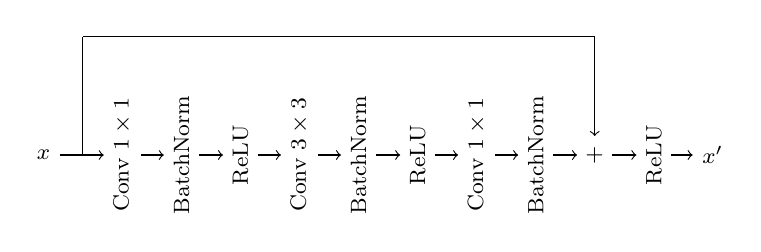
\begin{tikzpicture}[]
    % Nodes
    \node at (0,0) (input){\footnotesize$x$};
    \node[align=center] (conv1) at (1, 0) {\rotatebox{90}{\footnotesize\Th{Conv} $1\times1$}};
    \node[align=center] (bn1) at (1.75, 0) {\rotatebox{90}{\footnotesize\Th{BatchNorm}}};
    \node[align=center] (relu1) at (2.5, 0) {\rotatebox{90}{\footnotesize\Th{ReLU}}};
    \node[align=center] (conv2) at (3.25, 0) {\rotatebox{90}{\footnotesize\Th{Conv} $3\times3$}};
    \node[align=center] (bn2) at (4, 0) {\rotatebox{90}{\footnotesize\Th{BatchNorm}}};
    \node[align=center] (relu2) at (4.75, 0) {\rotatebox{90}{\footnotesize\Th{ReLU}}};
    \node[align=center] (conv3) at (5.5, 0) {\rotatebox{90}{\footnotesize\Th{Conv} $1\times1$}};
    \node[align=center] (bn3) at (6.25, 0) {\rotatebox{90}{\footnotesize\Th{BatchNorm}}};
    \node[align=center] (sum) at (7, 0) {\rotatebox{90}{\footnotesize$+$}};
    \node[align=center] (relu3) at (7.75, 0) {\rotatebox{90}{\footnotesize\Th{ReLU}}};
    \node(output) at (8.5, 0) {\footnotesize$x'$};
    \node at (0.5, 0) (empt0) {};
    \node at (0.5, 1.5) (empt1) {};
    \node at (7, 1.5) (emptkek) {};  

    %% CNN Edges
    \draw[->] (input.east) -- node {} (conv1);
    \draw[->] (conv1.east) -- node  {} (bn1.west);
    \draw[->] (bn1.east) -- node  {} (relu1.west);
    \draw[->] (relu1.east) -- node  {} (conv2.west);
    \draw[->] (conv2.east) -- node  {} (bn2.west);
    \draw[->] (bn2.east) -- node  {} (relu2.west);
    \draw[->] (relu2.east) -- node  {} (conv3.west);
    \draw[->] (conv3.east) -- node  {} (bn3.west);
    \draw[->] (bn3.east) -- node  {} (sum.west); 
    \draw[-] (empt0.center) -| node {} (empt1.center);
    \draw[-] (empt1.center) -- node {} (emptkek.center);
    \draw[->] (emptkek.center) -- node {} (sum.north);
    \draw[->] (sum.east) -- node  {} (relu3.west);
    \draw[->] (relu3.east) -- node  {} (output.west);
\end{tikzpicture}
